\documentclass[11pt]{article}
%\usepackage[handout, nostamp]{moodle}
%\usepackage{catchfilebetweentags}
\usepackage[nostamp]{moodle}
\usepackage{graphicx}
\usepackage{comment}
\usepackage{fancyvrb}
\usepackage{geometry}
\pagestyle{empty}
 \geometry{
 a4paper,
 total={175mm,260mm},
 left=15mm,
 top=15mm,
 }

\begin{document}
\begin{quiz}{Reti sequenziali}


%**************************************************************************
%First circuit
%**************************************************************************

\begin{cloze}[points=1,shuffle=false]{Reti sequenziali}
    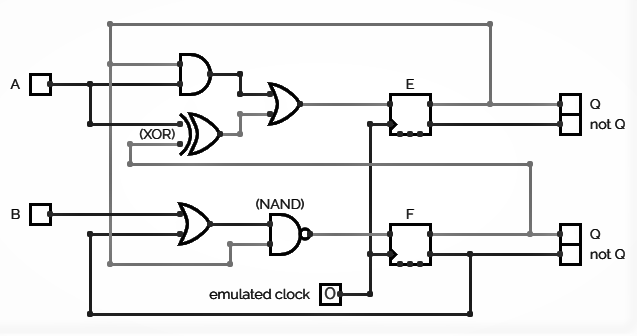
\includegraphics[height=9cm]{figures/seq_1.png}
    
    Data la rete sequenziale sincrona mostrata in figura, si supponga che i due flip-flop di tipo D,
    etichettati $E$ ed $F$, memorizzino inizialmente lo stato $(Q_E,Q_F) = (0,0)$.
    Assumendo inoltre che sugli ingressi vengano fissati i valori $(A,B)=(0,0)$,
    determinare:
    
    \begin{itemize}
    \item lo stato del flip-flop $E$ dopo 1 ciclo di clock \begin{shortanswer} \item 0 \end{shortanswer}
    \item lo stato del flip-flop $F$ dopo 1 ciclo di clock \begin{shortanswer} \item 1 \end{shortanswer}
    \item lo stato del flip-flop $E$ dopo 2 cicli di clock \begin{shortanswer} \item 1 \end{shortanswer}
    \item lo stato del flip-flop $F$ dopo 2 cicli di clock \begin{shortanswer} \item 1 \end{shortanswer}
    \end{itemize}
\end{cloze}
    
\begin{cloze}[points=1,shuffle=false]{Reti sequenziali}
    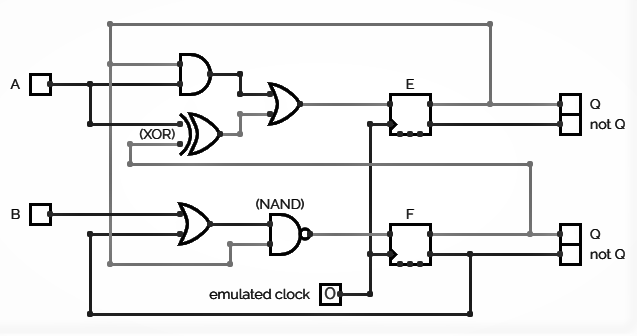
\includegraphics[height=9cm]{figures/seq_1.png}
    
    Data la rete sequenziale sincrona mostrata in figura, si supponga che i due flip-flop di tipo D,
    etichettati $E$ ed $F$, memorizzino inizialmente lo stato $(Q_E,Q_F) = (0,1)$.
    Assumendo inoltre che sugli ingressi vengano fissati i valori $(A,B)=(0,1)$,
    determinare:
    
    \begin{itemize}
    \item lo stato del flip-flop $E$ dopo 1 ciclo di clock \begin{shortanswer} \item 1 \end{shortanswer}
    \item lo stato del flip-flop $F$ dopo 1 ciclo di clock \begin{shortanswer} \item 1 \end{shortanswer}
    \item lo stato del flip-flop $E$ dopo 2 cicli di clock \begin{shortanswer} \item 1 \end{shortanswer}
    \item lo stato del flip-flop $F$ dopo 2 cicli di clock \begin{shortanswer} \item 0 \end{shortanswer}
    \end{itemize}
\end{cloze}

\begin{cloze}[points=1,shuffle=false]{Reti sequenziali}
    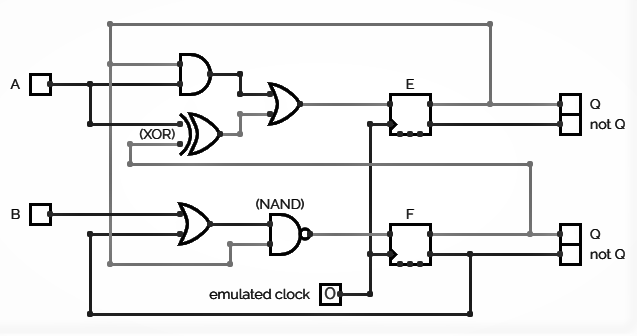
\includegraphics[height=9cm]{figures/seq_1.png}
    
    Data la rete sequenziale sincrona mostrata in figura, si supponga che i due flip-flop di tipo D,
    etichettati $E$ ed $F$, memorizzino inizialmente lo stato $(Q_E,Q_F) = (1,1)$.
    Assumendo inoltre che sugli ingressi vengano fissati i valori $(A,B)=(1,1)$,
    determinare:    
    \begin{itemize}
    \item lo stato del flip-flop $E$ dopo 1 ciclo di clock \begin{shortanswer} \item 1 \end{shortanswer}
    \item lo stato del flip-flop $F$ dopo 1 ciclo di clock \begin{shortanswer} \item 0 \end{shortanswer}
    \item lo stato del flip-flop $E$ dopo 2 cicli di clock \begin{shortanswer} \item 1 \end{shortanswer}
    \item lo stato del flip-flop $F$ dopo 2 cicli di clock \begin{shortanswer} \item 0 \end{shortanswer}
    \end{itemize}
\end{cloze}

%**************************************************************************
%Second circuit
%**************************************************************************

\begin{cloze}[points=1,shuffle=false]{Reti sequenziali}
    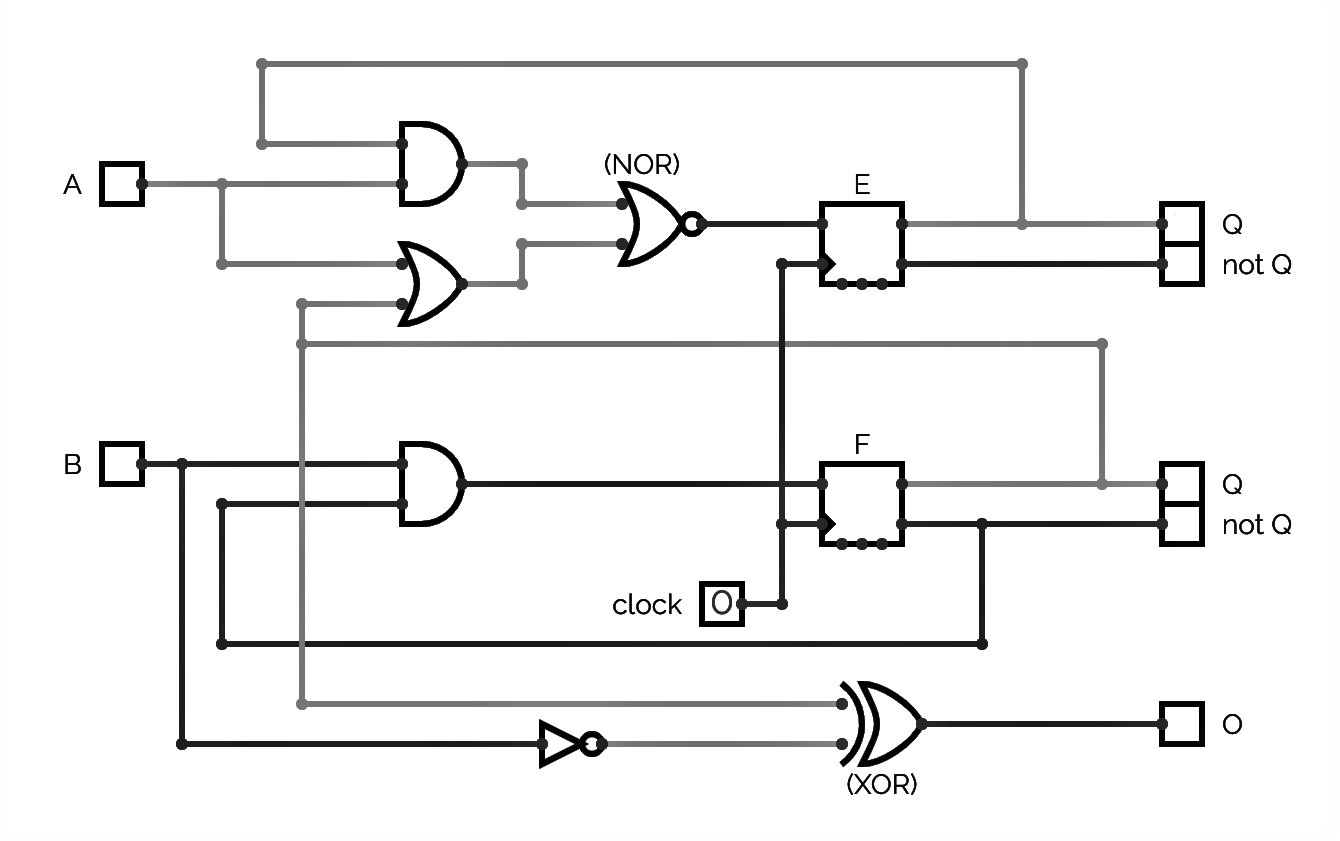
\includegraphics[height=9cm]{figures/seq_2.png}
    
    Data la rete sequenziale sincrona mostrata in figura, si supponga che i due flip-flop di tipo D,
    etichettati $E$ ed $F$, memorizzino inizialmente lo stato $(Q_E,Q_F) = (0,0)$.
    Assumendo inoltre che sugli ingressi vengano portati i valori $(A,B)=(0,0)$,
    determinare:
    
    \begin{itemize}
    \item lo stato futuro del flip-flop $E$ \begin{shortanswer} \item 1 \end{shortanswer}
    \item lo stato futuro del flip-flop $F$ \begin{shortanswer} \item 0 \end{shortanswer}
    \item il valore dell'uscita $O$ \begin{shortanswer} \item 1 \end{shortanswer}
    \end{itemize}
\end{cloze}


\begin{cloze}[points=1,shuffle=false]{Reti sequenziali}
    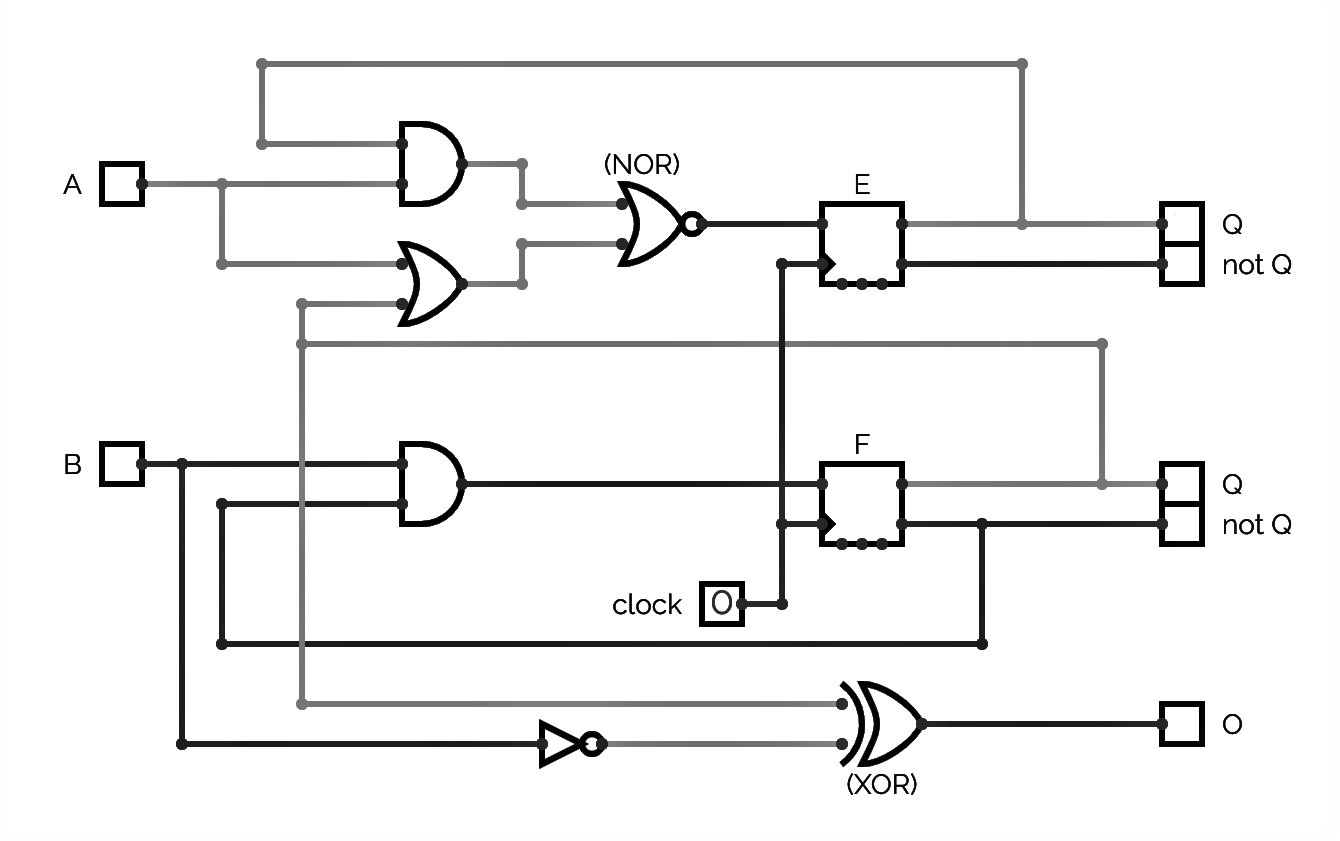
\includegraphics[height=9cm]{figures/seq_2.png}
    
    Data la rete sequenziale sincrona mostrata in figura, si supponga che i due flip-flop di tipo D,
    etichettati $E$ ed $F$, memorizzino inizialmente lo stato $(Q_E,Q_F) = (1,0)$.
    Assumendo inoltre che sugli ingressi vengano portati i valori $(A,B)=(0,0)$,
    determinare:
    
    \begin{itemize}
    \item lo stato futuro del flip-flop $E$ \begin{shortanswer} \item 1 \end{shortanswer}
    \item lo stato futuro del flip-flop $F$ \begin{shortanswer} \item 0 \end{shortanswer}
    \item il valore dell'uscita $O$ \begin{shortanswer} \item 1 \end{shortanswer}
    \end{itemize}
\end{cloze}

%**************************************************************************
%Third circuit
%**************************************************************************

\begin{cloze}[points=1,shuffle=false]{Reti sequenziali}
    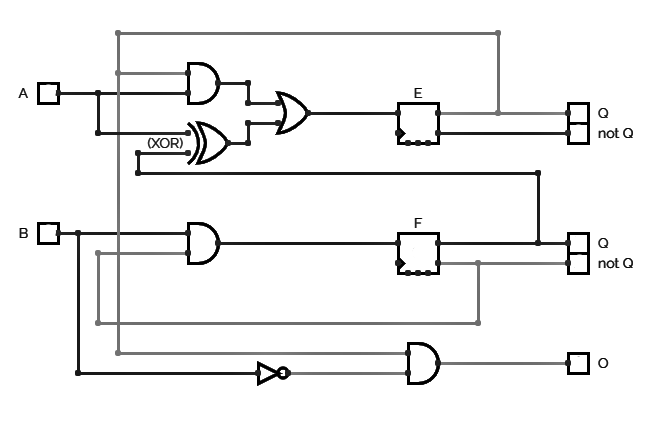
\includegraphics[height=9cm]{figures/seq_3.png}
    
    Data la rete sequenziale sincrona mostrata in figura, si supponga che i due flip-flop di tipo D,
    etichettati $E$ ed $F$, memorizzino inizialmente lo stato $(Q_E,Q_F) = (1,0)$.
    Assumendo inoltre che sugli ingressi vengano portati i valori $(A,B)=(0,1)$,
    determinare:
    
    \begin{itemize}
    \item lo stato futuro del flip-flop $E$ \begin{shortanswer} \item 0 \end{shortanswer}
    \item lo stato futuro del flip-flop $F$ \begin{shortanswer} \item 1 \end{shortanswer}
    \item il valore dell'uscita $O$ \begin{shortanswer} \item 0 \end{shortanswer}
    \end{itemize}
\end{cloze}

\begin{cloze}[points=1,shuffle=false]{Reti sequenziali}
    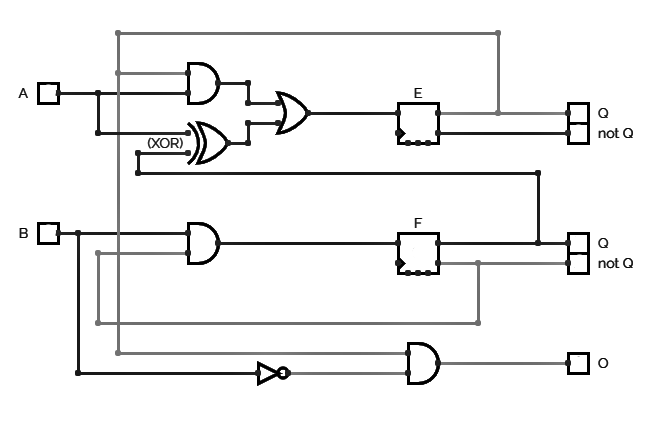
\includegraphics[height=9cm]{figures/seq_3.png}
    
    Data la rete sequenziale sincrona mostrata in figura, si supponga che i due flip-flop di tipo D,
    etichettati $E$ ed $F$, memorizzino inizialmente lo stato $(Q_E,Q_F) = (0,1)$.
    Assumendo inoltre che sugli ingressi vengano portati i valori $(A,B)=(0,1)$,
    determinare:
    
    \begin{itemize}
    \item lo stato futuro del flip-flop $E$ \begin{shortanswer} \item 1 \end{shortanswer}
    \item lo stato futuro del flip-flop $F$ \begin{shortanswer} \item 0 \end{shortanswer}
    \item il valore dell'uscita $O$ \begin{shortanswer} \item 0 \end{shortanswer}
    \end{itemize}
\end{cloze}

\end{quiz}
\end{document}